%-----------------------------------------------------------------------
%
%     This file is part of the Code_Saturne Kernel, element of the
%     Code_Saturne CFD tool.
%
%     Copyright (C) 1998-2008 EDF S.A., France
%
%     contact: saturne-support@edf.fr
%
%     The Code_Saturne Kernel is free software; you can redistribute it
%     and/or modify it under the terms of the GNU General Public License
%     as published by the Free Software Foundation; either version 2 of
%     the License, or (at your option) any later version.
%
%     The Code_Saturne Kernel is distributed in the hope that it will be
%     useful, but WITHOUT ANY WARRANTY; without even the implied warranty
%     of MERCHANTABILITY or FITNESS FOR A PARTICULAR PURPOSE.  See the
%     GNU General Public License for more details.
%
%     You should have received a copy of the GNU General Public License
%     along with the Code_Saturne Kernel; if not, write to the
%     Free Software Foundation, Inc.,
%     51 Franklin St, Fifth Floor,
%     Boston, MA  02110-1301  USA
%
%-----------------------------------------------------------------------
\section{SOLUTION FOR CASE 3}

Only a few elements are different from case 2.

In this case the density becomes variable. Go to the item
{\itshape Fluid properties} under the heading
{\itshape Physical properties} and change the nature of the density from
{\itshape constant} to {\itshape variable}.

\begin{figure}[h!]
\begin{center}
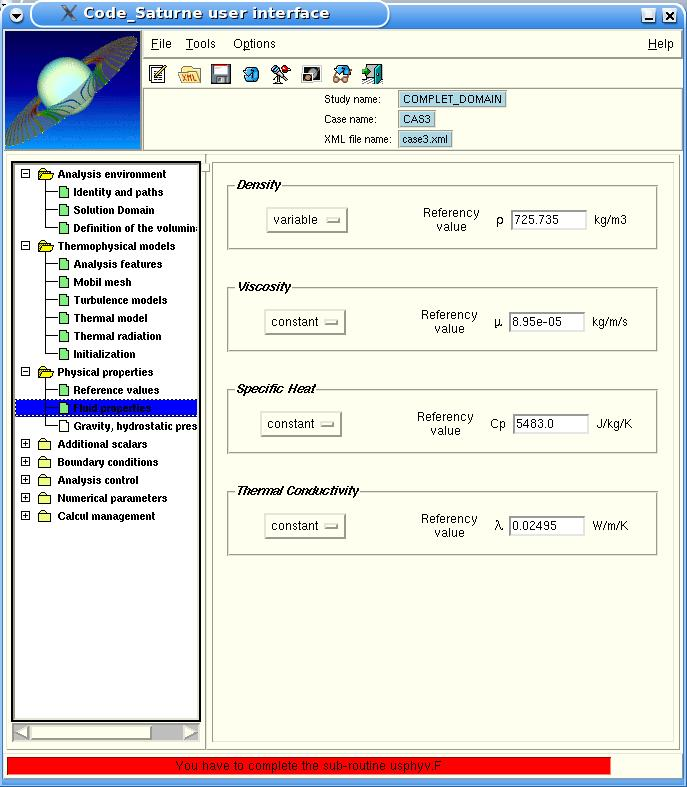
\includegraphics[width=12cm]{\repgraphics/c3_capture01.jpg}
\caption{Fluid properties - Variable density}
\label{fig1_e3}
\end{center}
\end{figure}


\newpage
As the density is variable, the influence of gravity has to be considered. In the
heading {\itshape Physical properties} go to
{\itshape Gravity, hydrostatic pressure} and set the value of each component of
the gravity vector. If the norm of gravity is the standard $9.81\ m.s^{-2}$, a
alternative way to define gravity is to specify its direction in the component
boxes, (0;-1;0) in our case, and click on the icon below to renormalize the
vector to 9.81.

\begin{figure}[h!]
\begin{center}
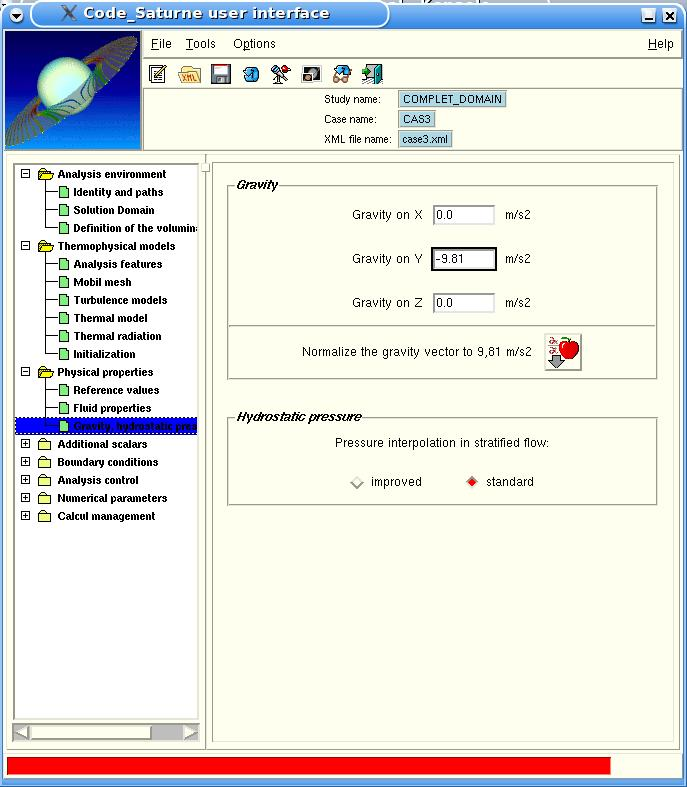
\includegraphics[width=12cm]{\repgraphics/c3_capture02.jpg}
\caption{Fluid properties - Gravity}
\label{fig2_e3}
\end{center}
\end{figure}


\newpage
Add a monitoring point close to the entry boundary condition in the
{\itshape Output control} item.

\begin{center}
\begin{tabular}{|c|c|c|c|}
\hline
Points & X(m) & Y(m) & Z(m)\\
\hline
9 & -0.5 & 2.25 & 0 \\
\hline
\end{tabular}
\end{center}

\begin{figure}[h!]
\begin{center}
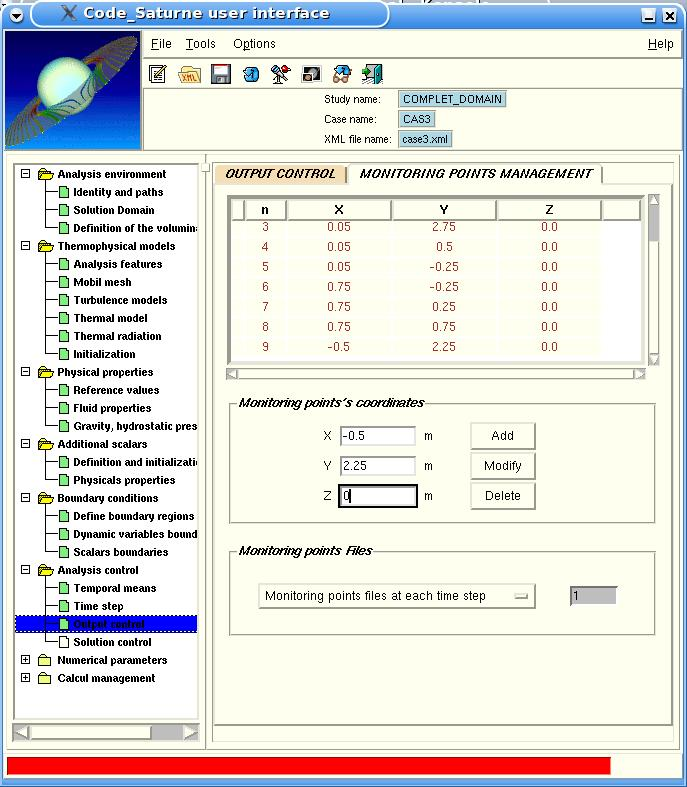
\includegraphics[width=12cm]{\repgraphics/c3_capture03.jpg}
\caption{New monitoring probe}
\label{fig3_e3}
\end{center}
\end{figure}


\newpage
After completing the interface, before running the calculation,
some Fortran user routines need to be modified.

Go to the folder FORT/USERS/base and copy {\itshape usclim.F} and
{\itshape usphyv.F} in the FORT directory.

$\bullet\ $\textbf{usclim.F}\\
In this case, {\itshape usclim.F} is used to specify the time dependent boundary
condition for
the temperature. Refer to the comments in the routine or to the \CS user manual
for more information on this routine.\\
In our case, you need to identify the boundary faces of color 1. The command\\
CALL GETFBR('1',NLELT,LSTELT)
will return an integer NLELT, corresponding to the number of boundary faces of
color 1, and an integer array LSTELT containing the list of the NLELT boundary
faces of color 1. Note that the string '1' can be more complex and combine
different colors, group references or geometrical criteria, with the same syntax
as in the Graphical Interface.

For each boundary face IFAC in the list, the Dirichlet value is given in the
multi-dimension array RCODCL as follows:
\begin{verbatim}
IF (TTCABS.LT.3.8D0) THEN
  DO IELT = 1, NLELT
    IFAC = LSTELT(IELT)
    RCODCL(IFAC,ISCA(1),1) = 20.D0+100.D0*TTCABS
  ENDDO
ELSE
  DO IELT = 1, NLELT
    IFAC = LSTELT(IELT)
    RCODCL(IFAC,ISCA(1),1) = 400.D0
  ENDDO
ENDIF
\end{verbatim}
ISCA(1) refers to the first scalar and TTCABS is the current physical time.

See the example file in the directory TEST\_CASES for the complete
{\itshape usclim.F} file.

Note that, although the inlet boundary conditions for temperature are specified
in the {\itshape usclim.F} file, it is necessary to specify them also in the
Graphical Interface. The value given in the Interface can be anything, it will
be overwritten by the Fortran routine.


$\bullet\ $\textbf{usphyv.F}\\
In this case, {\itshape usphyv.F} is used to specify the law that governs the
variation of density as a function of the temperature. The physical
characteristics at the center of the cells are stored in the array PROPCE
(respectively PROPFA for the internal faces and PROPFB for the boundary faces).
The index of the physical characteristic ``density'' among the other
characteristics is IROM(IPHAS) for the phase IPHAS.
Not all the physical characteristics are stored at the center of the cells and
some characteristics are stored both at the centers of the cells and on the
boundary faces, for instance.
Therefore, another array is used, to specify, for a given physical
characteristics stored at the centers of the cells, its index among the other
physical characteristics stored at the centers of the cells. It is the array
IPPROC (IPPROF for the internal faces and IPPROB for the boundary faces).\\
Hence, the fluid density at the center of cell IEL, for phase IPHAS(=1) is:\\
PROPCE(IEL,IPPROC(IROM(IPHAS)))

It is this array that has to be modified. The variable density in the cell IEL
is calculated from the fluid temperature in this cell, stored in\\
RTP(IEL,ISCA(1))

See the example file in the directory TEST\_CASES for the complete
{\itshape usphyv.F} file.


After updating these two Fortran files, run the calculation as explained in case
2.


\newpage
When a calculation is finished, \CS stores all the necessary elements to
continue the computation in another execution, with total continuity. These
elements are stored in several files, grouped in a SUITE.xxxxxxxx directory, in
the RESU directory.

In this case, after the first calculation is finished, a second calculation will
be run, starting from the results of the first one.


Go directly on the item {\itshape Start/Restart} under the heading
{\itshape Calcul management}.  Activate the {\itshape Analysis restart}
by ticking the ``on'' box. Then click on the folder icon next to it to specify
the restart files to use.

\begin{figure}[h!]
\begin{center}
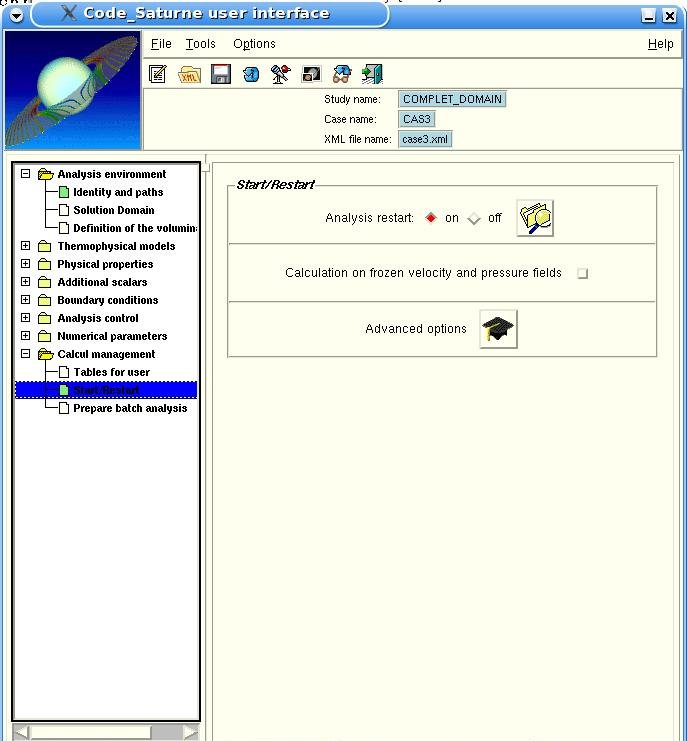
\includegraphics[width=12cm]{\repgraphics/c3_capture04.jpg}
\caption{Start / Restart}
\label{fig4_e3}
\end{center}
\end{figure}


\newpage
A window opens, with the architecture of the study sub-directories. Open the
RESU folder and click on the folder SUITE.xxxxxxxx (where xxxxxxxx corresponds
to the reference of the first calculation). Then click on {\itshape Validate}.

\begin{figure}[h!]
\begin{center}
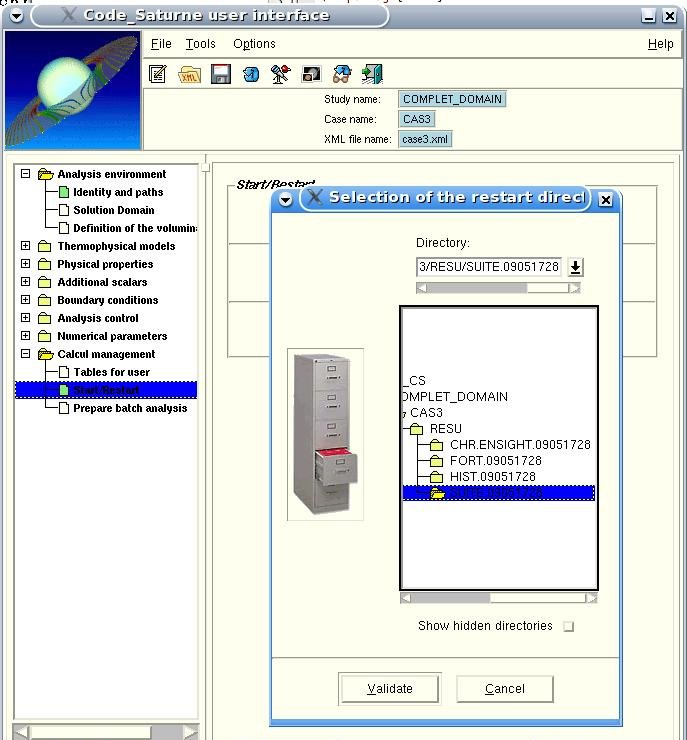
\includegraphics[width=12cm]{\repgraphics/c3_capture05.jpg}
\caption{Start / Restart - Selection of the restart directory}
\label{fig5_e3}
\end{center}
\end{figure}


\newpage
Go to the {\itshape Time step} item under the heading {\itshape Analysis
control} and change the number of iterations. It must be the total number of
iterations, from the beginning of the first calculation.\\

The first calculation was done with 300 iterations and another 400 iterations
are needed for the present case. Therefore the value 700 must be entered.

\begin{figure}[h!]
\begin{center}
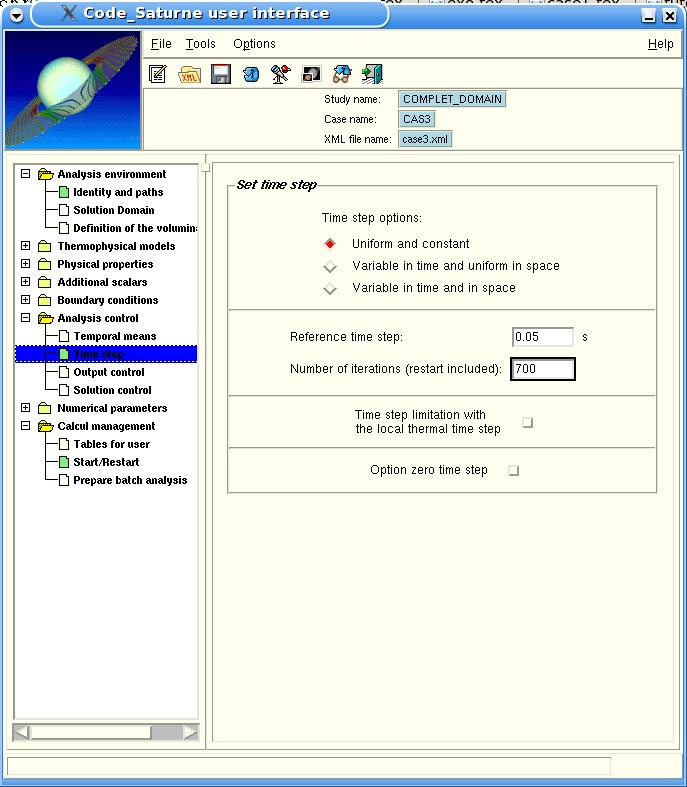
\includegraphics[width=12cm]{\repgraphics/c3_capture06.jpg}
\caption{Time step}
\label{fig6_e3}
\end{center}
\end{figure}

Eventually, run the calculation.
